\documentclass{beamer}

\usepackage{helvet}
\usepackage{hyperref, graphicx}
\usepackage{amsthm, amsfonts}
\usepackage{etoolbox}
%\usepackage{multicol}
%\usepackage{tikz}
\usepackage{caption}
\usepackage{ulem}

%% Define the layout of slides, numbering, and color theme
%% Also, make links in TOC appear at start of each section 
\usetheme[progressbar=frametitle, numbering=none]{metropolis}
\usecolortheme[snowy]{owl}
\setbeamertemplate{navigation symbols}{}
\AtBeginSection[ ]
{
\begin{frame}{Outline}
    \tableofcontents[currentsection]
\end{frame}
}

%% Default fixed font does not support bold face
\DeclareFixedFont{\ttb}{T1}{txtt}{bx}{n}{11} % for bold
\DeclareFixedFont{\ttm}{T1}{txtt}{m}{n}{12}  % for normal - use in headings

%% Custom colors
\usepackage{color}
\definecolor{TUGray}{RGB}{101,101,137}
\definecolor{TUBlack}{RGB}{0,0,10}
\definecolor{mygreen}{RGB}{45,111,63}
\definecolor{keywords}{RGB}{205,114,0}
\definecolor{comments}{RGB}{181,51,139}
\definecolor{strings}{RGB}{58,144,81}
\definecolor{numeric}{RGB}{66,110,176}
\definecolor{linos}{rgb}{0.4,0.4,0.4}
\definecolor{links}{rgb}{0,0.4,0.75}

\definecolor{bggray}{RGB}{232, 233, 235}

\setbeamercolor{alerted text}{fg=mygreen}
\setbeamercolor{normal text}{fg=TUBlack}\usebeamercolor*{normal text}

\setbeamercolor{codecol}{fg=TUGray!25!black,bg=bggray}

%% Coloring of links
\hypersetup{colorlinks, linkcolor=links, urlcolor=links}

%% Custom multi-line commenting out
\newcommand{\comment}[1]{}

%% Fonts
\usepackage[T1]{fontenc}
\usepackage[sfdefault,scaled=.85]{FiraSans}
\usepackage{newtxsf}

%% Package for displaying lines of code, or pseudocode
\usepackage{listings}

\newtoggle{InString}{}% Keep track of if we are within a string
\togglefalse{InString}% Assume not initally in string

%% Some line parsing in listings code blocks, to perform highlighting (digits,keywords, comments, etc)
\newcommand\digitstyle{\color{numeric}}
\makeatletter
\newcommand{\ProcessDigit}[1]
{%
  \ifnum\lst@mode=\lst@Pmode\relax%
   {\digitstyle #1}%
  \else
    #1%
  \fi
}
\makeatother

\lstset{literate=%
    {0}{{{\ProcessDigit{0}}}}1
    {1}{{{\ProcessDigit{1}}}}1
    {2}{{{\ProcessDigit{2}}}}1
    {3}{{{\ProcessDigit{3}}}}1
    {4}{{{\ProcessDigit{4}}}}1
    {5}{{{\ProcessDigit{5}}}}1
    {6}{{{\ProcessDigit{6}}}}1
    {7}{{{\ProcessDigit{7}}}}1
    {8}{{{\ProcessDigit{8}}}}1
    {9}{{{\ProcessDigit{9}}}}1
	{<=}{{\(\leq\)}}1
	{>=}{{\(\geq\)}}1,
	% morestring=[b]",
    % morestring=[b]',
    % morecomment=[l]{//},
}

%% Defining keywords and comment formatting for a pseudocode block
\lstdefinelanguage{Pseudo}{
    morekeywords={return, while, if, for, input},
    morecomment=[l]{\#},
}

%% Pseudocode style
\newcommand\pseudostyle{\lstset{
language=Pseudo,
basicstyle=\fontfamily{ccr}\scriptsize,
commentstyle=\it\scriptsize\color{linos},
keywordstyle=\it\bfseries\scriptsize,
mathescape=true,
literate=
    {=}{$\leftarrow{}$}{1}
    {==}{$={}$}{1}
    {<=}{{\(\leq\)}}1
	{>=}{{\(\geq\)}}1,
xleftmargin=18pt,
xrightmargin=4pt,
aboveskip=12pt,
belowskip=0pt,
frame=tB,
keepspaces=true
}}

%% Python style
\newcommand\pythonstyle{\lstset{
language=Python,
basicstyle=\ttfamily\tiny,
numbers=left,
numberstyle=\tiny\color{linos},
morekeywords={self, np},              % Add keywords here
keywordstyle=\tiny\color{keywords},
commentstyle=\it\tiny\color{comments},    % Custom highlighting style
stringstyle=\tiny\color{strings},
xleftmargin=18pt,
xrightmargin=4pt,
aboveskip=0pt,
belowskip=0pt,
escapeinside={(*@}{@*)},
frame=l,                         % Any extra options here
showstringspaces=false,
keepspaces=true
}}

%% Pseudocode environment
\lstnewenvironment{pseudo}[1][]
{
    \pseudostyle
    \lstset{
        #1
    }
}
{}

%% Python environment 
\lstnewenvironment{python}[1][]
{
	\pythonstyle
	\lstset{
	#1
	}
}
{}

%% wrap the Python environment
\newenvironment{codeblock}
    {\hfill\begin{beamerboxesrounded}[lower=codecol, width=0.8\textwidth]
    \medskip

    }
    { 
    \end{beamerboxesrounded}\hfill
    }

%% A couple of block enviroments to make statement stand out
\theoremstyle{example}
\newtheorem{question}{Question}

%% Some shortcut macros for computer-type font
\newcommand{\ct}[1]{\lstinline[language=Python]!#1!}
\newcommand{\st}[1]{\lstinline[language=Python,basicstyle=\ttfamily,stringstyle=\small\color{strings}]!#1!}
\newcommand{\ttt}[1]{{\small\texttt{#1}}}
\newcommand{\lsitem}[2]{\ttt{{#1}[}\ct{#2}\ttt{]}}
\newcommand{\bb}[1]{\mathbb{#1}}
\newcommand{\cl}[1]{\mathcal{#1}}
\newcommand{\gnum}[1]{{\color{mygreen}#1.}}

%% Header information
\author{Chris Cornwell}
\date{Aug 26, 2025}
\title{Pipeline of Machine Learning}

%% Start of slides
\begin{document}

\begin{frame}
\titlepage
\end{frame}

\begin{frame}
\frametitle{Outline}
\tableofcontents
\end{frame}

\section{The Pipeline}

%% ML Pipeline
%%%%
\begin{frame}
\frametitle{Steps in an ML Project}

\begin{codeblock}

{\color{mygreen}Project Pipeline
    \begin{enumerate}
        \item[\gnum{0}] Define the problem.
        \item[\gnum{1}] Collect data.
        \item[\gnum{2}] Design the features in the data.
        \item[\gnum{3}] Training of the model.
        \item[\gnum{4}] Test the model.
    \end{enumerate}
}

\end{codeblock}

\end{frame}

%%%%
\begin{frame}
\frametitle{Discussion on the ML Project Pipeline}
    \begin{enumerate}
        \item[\gnum{0}] Define the problem.
        \begin{itemize}
            \item Example: From a given image, determine if it is an image of a dog or not.
        \end{itemize}
        \pause
        \item[\gnum{1}] Collect data.
        \begin{itemize}
            \item Example: Put together a large collection of images, some having dogs in them, others having a different animal, or no animal. Have a label (your output, ``$y$'') for each image. Split into training set and test set.
        \end{itemize}
        \pause
        \item[\gnum{2}] Design the features in the data.
        \begin{itemize}
            \item Not one thing that you always do here. Sometimes use experience/knowledge of what the data represents, sometimes use another learning algorithm to \textit{learn} good features.
        \end{itemize}
    \end{enumerate}
\end{frame}

%%%%
\begin{frame}
\frametitle{Discussion on the ML Project Pipeline}
    \begin{enumerate}
        \item[\gnum{3}] Training of the model.%Where we will spend a lot of time; lots of developed mathematics and algorithms.
        \begin{itemize}
            \item Model is determined by set of parameters. In training, you alter the parameters iteratively {--} ``tune'' them {--} using optimization techniques (on the loss function).
        \end{itemize}
        \item[\gnum{4}] Test the model.
        \begin{itemize}
            \item Evaluate the trained model's performance on test data, measured by the same loss function.
        \end{itemize}
    \end{enumerate}
\end{frame}

%%%%
\begin{frame}[standout]
    Poll question
\end{frame}

%%%%
\begin{frame}
\frametitle{Difficulty in Defining the Problem}
    Examples worked with when first learning ML have a easily defined problem (\textit{e.g.}, here are images of handwritten numbers; determine which number is written); defining problem harder in real practice.  
    \pause

    \begin{codeblock}
        \textcolor{mygreen}{Example.} Have database of Tweets (from X / Twitter) about news events; interested in using machine learning to determine which are giving misinformation.

        Is it a simple classification problem, {\small\st{'misinformation'}} vs. {\small\st{'not'}}? If not, what alternative is there?
    \end{codeblock}

    Sometimes the issue is in the data. 
    
    \begin{codeblock}
        \textcolor{mygreen}{Example.} Attempting to use crime data in Baltimore to model how crimes occur by location (\textit{e.g.}, reoccurrence of crime at same location shortly after).
    \end{codeblock}

\end{frame}

%%%%
\begin{frame}
\frametitle{Difficulty in Designing Features}
Very often, data is gathered in format or coordinates that make it hard to achieve ML task or, at least, do not help.

Will discuss some techniques that identify coordinates that ``do not help'' (Feature selection).

\pause
Domain knowledge is important for designing (computing) better features from given data.

\pause
\begin{codeblock}
        \textcolor{mygreen}{Example.} In textbook, reconstructed Galileo experiment for objects falling. 

        \begin{center}Force of gravity is constant ($g$) 
            
            $\Downarrow$ 
            
        height change is $\frac{g}{2}t^2$ (from Calculus)
        \end{center}
\end{codeblock}

\end{frame}

%%%%
\begin{frame}[standout]
    Poll question
\end{frame}

%%%%
\begin{frame}
\frametitle{Difficulty in Designing Features}
Some studies on brain function suggest that visually recognizing something is correlated with identifying edges in an image.

Computer vision learning algorithms are built to compute such edge features from input image.

\pause
\begin{center}
    \begin{tikzpicture}[>=stealth]
        \draw (0,0) node {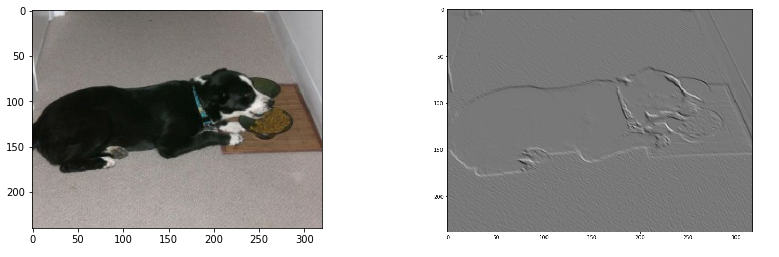
\includegraphics[width=\textwidth]{../../Images/filter-dogimage.png}};
        \draw[->,thick] (-0.4,0) -- (0.4,0);
    \end{tikzpicture}
\end{center}
\end{frame}

{\setbeamercolor{palette primary}{fg=mygreen, bg=bggray}
\begin{frame}[standout]
    Questions?
\end{frame}
}
\end{document}